% !TEX root = ../my_thesis.tex
\pagebreak
\section{Stand der Forschung und Grundlagen}

Dieses Kapitel versucht einen Überblick des Forschungsstandes in den unterschiedlichen Aspekten der Arbeit zu verschaffen. Anschließend vermittelt das Kapitel notwendige Grundkenntnisse.

\subsection{Einführung}


% SLAM, visual Odometrie, Viewpoint,

% Lokalisierungsproblem erläutern
% Ansätze aufzählen
% Überführen auf visuelle Lokalisierung
// Evt. Einblick über indoor Lokalizierungstechnicken \\

\textbf{Pose Estimation} wird in dieser Arbeit als eine Methode der visuellen Lokalisierung (\textit{Visual-Based Localization, kurz VBL}) betrachtet. VBL beschäftigt sich mit der Bestimmung der Pose (\textit{Position + Orientierung}) eines visuellen Abfragematerials (\textit{z.B. ein RGB-Bild}) in einer zuvor bekannten Szene  \cite{piascoSurveyVisualBasedLocalization2018}.
Ein naheliegendes Themengebiet der Robotik ist die visuelle Ortswiedererkennung (\textit{Visual Place Recognition, kurz VPR}) \cite{lowryVisualPlaceRecognition2016}. Die visuelle Ortswiedererkennung fokussiert sich auf das Feststellen eines bereits besuchten Ortes und definiert sich aus einer Mapping-, Datenverarbeitungs- und einem Orientierungsmodul. Allgemein lässt sich das Prozess eines VPRs folgend beschreiben. Eine interne Karte bekannter Orte wird durch das Mappingmodul verwaltet. Die Daten werden vom Datenverarbeitungsmodul vorbereitet und anschließend an das Orientierungsmodul übergeben. Daraufhin bestimmt das Orientierungsmodul die Pose und entscheidet mit der immer aktuell gehaltenen Karte, ob ein Ort bereits besucht wurde.  Im Vergleich zur VPR versucht die visuelle Lokalisierung eine Pose zu bestimmen und benötigt daher neben den zwei Modulen kein Mappingmodul.

% hat 2 katogiren..
Die rein visuellen Methoden des VBLs unterteilen sich in indirekte und direkte Methoden \cite{lowryVisualPlaceRecognition2016}. Die indirekten Methoden behandeln das Lokalisierungsproblem als eine Bildersuche in einer Datenbank, ähnlich wie das \textit{Content Based Image Retrieval} \cite{lewContentbasedMultimediaInformation2006} Problem. Dabei wird das Abfragebild über eine Ähnlichkeitsfunktion mit den Vergleichsbildern aus der Datenbank abgeglichen \cite{zhangImageBasedLocalization2006, arandjelovicThreeThingsEveryone2012, radenovicCNNImageRetrieval2016}. Diese Art von Methoden benötigen eine sehr große Bildergalerie (\textit{Datenbank}) und liefern Ergebnisse bei Fund eines korrespondierenden Bildes \cite{lowryVisualPlaceRecognition2016}. Hingen versuchen die direkten Methoden die Pose über eine Referenzumgebung zu bestimmen und benötigen meist daher keine große Bildergalerie  \cite{piascoSurveyVisualBasedLocalization2018}. Es gibt drei Arten der direkten Methoden: 
\begin{enumerate*}[label=\arabic*)]
	\item Abgleichen von Features zu Punktwolken (\textit{z.B. \cite{liWorldwidePoseEstimation2012}})
	\item Pose Regression mit Tiefenbilder (\textit{z.B. \cite{shottonSceneCoordinateRegression2013a}})
	\item Pose Regression nur mit Bildern (\textit{z.B. \cite{kendallPoseNetConvolutionalNetwork2015}})
\end{enumerate*}

Die erste Art von Methoden versucht die Pose zu bestimmen, indem die 2D-3D Korrespondenz über das Abgleichen von Features des Abfragebildes gegen die Deskriptoren der 3D-Punkte hergestellt werden \cite{irscharaStructurefrommotionPointClouds2009, liWorldwidePoseEstimation2012, svarmCityScaleLocalizationCameras2017}. Diese Vorgehensweise hat Ähnlichkeiten zu den indirekten Methoden und benötigt statt einer Bildergalerie eine repräsentative 3D-Punktwolke der Szene \cite{piascoSurveyVisualBasedLocalization2018}. Die zweite Art von Methoden bestimmt anhand von Tiefenbilder die Pose z.B. über Regression Forests \cite{shottonSceneCoordinateRegression2013a}, Randomize Ferns \cite{glockerRealTimeRGBDCamera2015}, Coarse-to-Fine Registierung \cite{santosMappingIndoorSpaces2016} oder Neuronale Netze \cite{massicetiRandomForestsNeural2016}. Diese Forschungsprojekte liefern mit 3D-Bildern gewünschte Resultate. Die Ergebnisse sind abhängig von 3D-Kameras, diese sind jedoch nicht verbreitet.

\textbf{Convolutional Neural Networks} (\textit{CNN}) werden erfolgreich im Bereich des Maschinelles Sehens, wie z.B. bei der Klassifizierung von Bildern \cite{krizhevskyImageNetClassificationDeep2012, simonyanVeryDeepConvolutional2014, heDeepResidualLearning2015} sowie bei der Objekterkennung \cite{girshickRichFeatureHierarchies2013, renFasterRCNNRealTime2015b, girshickFastRCNN2015} eingesetzt. 
Ein verbreiteter Ansatz beim Entwurf von CNNs ist das häufige Feintunen (\textit{fine-tune}) der Netzwerkarchitekturen, die z.B. für die Bildklassifizierung angesichts der Aufgaben von ImageNet \cite{russakovskyImageNetLargeScale2014} konstruiert wurden. Dieser Ansatz konnte beispielsweise erfolgreich in der Objekterkennung \cite{girshickFastRCNN2015}, Objektsegmentierung \cite{kokkinosPushingBoundariesBoundary2015, maninisConvolutionalOrientedBoundaries2016}, semantische Segmentierung \cite{nohLearningDeconvolutionNetwork2015, hazirbasFuseNetIncorporatingDepth2017a} und Tiefenbestimmung \cite{liDepthSurfaceNormal2015} verfolgt werden.
Seit Kurzem werden CNNs auch in den Anwendungsgebieten der Lokalisierung verwendet. Zum Beispiel verwenden  \citet{parisottoGlobalPoseEstimation2018} CNNs in Bezug auf das Simultaneous-Localization-and-Mapping (\textit{SLAM}) Problem. \citet{melekhovRelativeCameraPose2017} schätzen anhand CNNs die relative Pose zweier Kameras. \citet{costanteExploringRepresentationLearning2016} und \citet{wangDeepVOEndtoendVisual2017} setzen es im Bereich der visuellen Odometrie ein.

% Posenet überführen & erklären
Geleitet von den \textit{state-of-the-art} Lokalisierungsergebnissen der CNNs stellen \citet{kendallPoseNetConvolutionalNetwork2015} den ersten Ansatz zu direkten Posebestimmung nur mit RGB-Bildern vor. PoseNet ist die Modifikation der GoogLeNet \cite{szegedyGoingDeeperConvolutions2015} Architektur und zweckentfremdet es von der Bildklassifizierung zu einem Pose-Regressor. Trainiert mit einem Datensatz, bestehend aus Paaren von Farbbild und Pose, kann es die sechs Freiheitsgrade der Kamerapose in unbekannten Szenen mittels eines Bildes bestimmen. Dieser Ansatz benötigt weder eine durchsuchbare Bildgalerie noch eine Punktwolke oder Tiefenbilder der Szene. Im Vergleich zu den metrischen Ansätzen wie SLAM oder visuelle Odometrie liefert es eine weniger akkurate Pose. Es bietet jedoch eine hohe Toleranz gegenüber Skalierungs- und Erscheinungsänderungen des Anfragebildes an \cite{piascoSurveyVisualBasedLocalization2018}.

% Varianten aufzählen
Es gibt mehrere Ansätze, die die Genauigkeit von PoseNet übertreffen.
Einen Fortschritt erhalten die Autoren von PoseNet durch die hier \cite{kendallModellingUncertaintyDeep2015a} vorgestellte Anpassung ihres Models an einem Bayessian Neural Network \cite{denkerTransformingNeuralNetOutput1991, mackayPracticalBayesianFramework1991}.
Dieselben Autoren erweitern PoseNet mit einer neuen Kostenfunktion unter Berücksichtigung von geometrischen Eigenschaften \cite{kendallGeometricLossFunctions2017}. \citet{walchImagebasedLocalizationUsing2016} und \citet{clarkVidLocDeepSpatioTemporal2017} setzen Long-Short-Term-Memory (\textit{LSTM}) \cite{hochreiterLongShortTermMemory1997a} Einheiten ein, um Wissen aus der Korrelation von Bildsequenzen zu gewinnen. \citet{wuDelvingDeeperConvolutional2017} und \citet{naseerDeepRegressionMonocular2017} augmentieren den Trainingsdatensatz. \citet{wuDelvingDeeperConvolutional2017} stocken den vorhandenen Datensatz auf, indem sie die Bilder künstlich rotieren. \citet{naseerDeepRegressionMonocular2017} erweitern zuerst über ein weiteres CNN den Datensatz um Tiefenbildern. Anschließend simulieren die Autoren RGB-Bilder aus verschiedenen Viewpoints. Im Vergleich zu PoseNet verwenden \citet{mullerSQUEEZEPOSENETIMAGEBASED2017} und \citet{melekhovImageBasedLocalizationUsing2017} eine andere Architektur. 
Das Modell von \citet{mullerSQUEEZEPOSENETIMAGEBASED2017} basiert auf die SqueezeNet \cite{iandolaSqueezeNetAlexNetlevelAccuracy2016} Architektur. \citet{melekhovImageBasedLocalizationUsing2017} stellen HourglassNet, basierend auf einem symmetrischen Encoder-Decoder Architektur, vor. \citet{brahmbhattGeometryAwareLearningMaps2018} und \citet{valadaDeepAuxiliaryLearning2018, valadaIncorporatingSemanticGeometric} binden zusätzliche Informationen wie z.B. visuelle Odometrie, GPS oder IMU ein. 

Jedes dieser Ansätze benötigen annotierte Traininsdaten. Für die Erstellung solcher Daten wurden beispielsweise mit entsprechender Hardware ausgerüstete Trolleys \cite{huitlTUMindoorExtensiveImage2012}, 3D-Kameras \cite{izadiKinectFusionRealtime3D2011} oder SfM-Methoden \cite{kendallPoseNetConvolutionalNetwork2015} eingesetzt.

% Simulierte 3D-Daten 
\textbf{Simulierte 3D-Daten} werden in der Literatur oft eingesetzt, um das manuelle Erzeugen und Annotieren von Daten umzugehen. \citet{pishchulinArticulatedPeopleDetection2012a}, \citet{pengLearningDeepObject2014}, \citet{suRenderCNNViewpoint2015} und \citet{varolLearningSyntheticHumans2017} erzeugen ihren Trainingsdaten, indem sie virtuelle Objekte auf reale Hintergrundbildern platzieren. \citet{pishchulinArticulatedPeopleDetection2012a} generieren Daten zwecks Personenerkennung und Bestimmung derer körperlicher Pose. Zuvor werden auf den vorhandenen Bildern die körperliche Pose der Personen bestimmt und daran deren 3D Modelle rekonstruiert. Anschließend werden die 3D-Modelle in ihrer Pose variiert auf reale Hintergrundbildern platziert. Die Autoren konnten vergleichbare Ergebnisse zu den vorhandenen Ansätzen mit realen Daten ermitteln. \citet{pengLearningDeepObject2014} erstellen Daten, um Objekte auf realen Bildern zu detektieren. Von jeder Objektklasse werden 3D-Modelle auf einem Hintergrundbild aus einer Sammlung gelegt. Die Autoren stellen fest, dass das Feintunen mit synthetischen Daten eines Netzwerkes dann zu Abnahme der Akkuratesse führt, wenn das Netzwerk \textit{nur} für die Detektierung eines Objektes bestimmt ist. Hingegen konnten sie eine Steigung der Ergebnisse beim Trainieren mit simulierten Daten auf vortraniertem Netzwerk mit einer größeren Klassifierungskatalog ermitteln. \citet{suRenderCNNViewpoint2015} generieren einen großen Datensatz mit 3D-Modellen, um den Viewpoint von Objekten auf realen Bildern zu bestimmen. Bei dieser Datengenerierung wird jedes virtuelle Objekt auf zufällige Hintergrundbildern positioniert und mit unterschiedlichen Konfigurationen (\textit{z.B. Beleuchtung}) gerendert. Die Autoren konnten mit der Datenaugmentierung \textit{state-of-the-art} Viewport-Estimation Methoden zur \textit{PASCAL 3D+}\cite{xiangPASCALBenchmark3D2014} Benchmark übertreffen. \citet{varolLearningSyntheticHumans2017} erstellen künstliche Personen auf Bildern, um beispielsweise den menschlichen Körper in seine Glieder zu segmentieren. Dabei rendern sie zufällige virtuelle Personen mit zufälliger Pose auf beliebige Hintergrundbildern und konnten zeigen, dass die Akkuratesse einiger CNNs durch das Trainieren mit den erzeugten Daten steigt. \citet{fanelloLearningBeDepth2014} rendert künstliche Infrarotbilder von Händen sowie Gesichtern zwecks Tiefenerkennung und Segmentierung der Hand in den einzelnen Fingern sowie des Gesichtes in Bereiche aus einem RGB-Bild. Die Autoren konnten konventionelle Methoden über  Helligkeitsabfall übertreffen und vergleichbare Ergebnisse zu den Ansätzen mit einer herkömmlichen 3D-Kamera erzielen. \citet{dosovitskiyFlowNetLearningOptical2015} erlernen mit synthetischen Daten den optischen Fluss von Bildsequenzen.  Hierbei werden auf Hintergrundbildern aus einer Sammlung mehrmals bewegte virtuelle Stühle platziert. Die Autoren konnten mit syntethischen Daten \textit{state-of-the-art} Ansätze über reale Daten übertreffen.

Motiviert von der Datengenerierung über 3D-simulierten Daten stellt \citet{haImagebasedIndoorLocalization2018} einen Ansatz zur bildbasierte Lokalisierung in Gebäuden vor. Dieser Forschungsansatz generiert synthetische Daten aus einem Building-Information-Modeling (\textit{BIM}). Bei den Daten werden die durch das vortrainierte VGG Netzwerk \cite{simonyanVeryDeepConvolutional2014} extrahierte Features als wesentlich erachtet und in einer Datenbank gepflegt. Ein reales Aufnahmebild im Gebäude lässt sich durch den Vergleich der Features lokalisieren. \citet{acharyaBIMPoseNetIndoorCamera2019, acharyaMODELLINGUNCERTAINTYSINGLE2019} erzeugen ebenso Trainingsdaten aus einem BIM, jedoch verwenden sie zur Lokalisierung keine Datenbank bedürftiges Verfahren, sondern bestimmen die Pose direkt über PoseNet. Die Daten werden entlang einer ca. 30$m$ langem Flugbahn aus der Simulation eines ca. 230$m^2$  Korridors gesammelt. Hierbei werden sich in der Realitätstreue vom \begin{enumerate*}[label=\alph*)]
	\item karikaturistisch zu
	\item fotorealistisch hin über zu
	\item fotorealistisch-texturiert
\end{enumerate*} unterscheidende Daten erzeugt.
Traniert mit den unterschiedlichen synthetischen Daten, getestet auf die realen Daten, erzielen die Forscher eine Akkuratesse von
\begin{enumerate*}[label=\alph*)]
	\item 6,25$m$
	\item 5,99$m$
	\item 3,06$m$
\end{enumerate*}
 in der Position und  
 \begin{enumerate*}[label=\alph*)]
 	\item 37,16°
 	\item 11,33°
 	\item 12,25°
 \end{enumerate*}
 in der Orientierung.
Die besten Ergebnisse konnten die Autoren trainiert mit den 
\begin{enumerate*}[label=\alph*)]
	\addtocounter{enumi}{3}
	\item Gradienten- und
	\item Kantenbilder
\end{enumerate*} der karikaturistischen Daten, getestet auf die Gradientenbilder der realen Aufnahmen, erzielen. Die Autoren erhalten eine Akkuratesse von 
\begin{enumerate*}[label=\alph*)]
	\addtocounter{enumi}{3}
	\item 2,63$m$
	\item 1,88$m$
\end{enumerate*}
in der Position und  
 \begin{enumerate*}[label=\alph*)]
 	\addtocounter{enumi}{3}
	\item 6,99°
	\item 7,73°
\end{enumerate*}
in der Orientierung.
\\\\// Anbindung zu meinem Beitrag
\\\\
Im weiteren Verlauf des Kapitels werden einige grundlegende Themen erläutert. Zuerst werden künstliche neuronale Netze definiert. Danach wird ein elementares Wissen an Convolutional Neural Networks vermittelt und anschließend bekannte CNN Modelle näher erläutert.

%\subsection{Lineare Faltung}
%\subsubsection{Sobelfilter}
%\subsubsection{Gradientenbild}
%Bei der Erzeugung von Gradienten- bzw. Kantenbilder gehen einerseits wichtige Informationen im Hinblick auf das Ursprungsbild verloren, andererseits bleiben wichtige Informationen wie z.B. die geometrische Struktur erhalten.

\subsection{Künstliche neuronale Netzwerke}
\label{sec:KNN}
Künstliche neuronale Netze sind ein Forschungsgebiet der \textit{künstlichen Intelligenz} und imitieren die Beschaffenheit natürlicher neuronale Netze, um komplexe Probleme zu lösen. Inspiriert von ihren biologischen Vorbildern \footnote{das Nervensystem eines Lebewesen, z.B. des Menschen}, vernetzen künstliche neuronale Netzwerke (\textit{KNN}) künstliche Neuronen miteinander \cite{CS231nConvolutionalNeural}. Dabei kann die Verbindung unidirektional (\textit{feedforward}) oder bidirektion (\textit{feedback}) sein. 

Bei einem feedforward Netzwerk werden die Daten im Netz immer vorwärts übertragen, hingegen kann ein \textit{feedback} Netzwerk, auch bekannt als \textit{Recurrent Neural Networks}, Daten rückwärts, sowie in einer Schleife zum selben Neuron, übergeben \cite{Goodfellow-et-al-2016}. Da feedback Netzwerke keinen Einsatz in dieser Arbeit haben, ist im weiteren Verlauf dieser Arbeit bei einem Netzwerk immer ein feedforward Ansatz gemeint.


\subsubsection{Künstliches Neuron}
Ein einzelnes Neuron erhält einen Inputsignal auf mehreren Kanälen und löst erst ein Signal (\textit{output}) aus, falls die gewichtete Summe des Inputs einen gewissen Schwellwert erreicht \cite{CS231nConvolutionalNeural}. Abbildung \ref{fig:neuron} stellt eine beispielhafte Visualisierung eines künstlichen Neurons dar.

Ein künstliches Neuron mit der Inputsgröße $M$ ist mathematisch die nicht-lineare Funktion $y : \mathbb{R}^M \mapsto \mathbb{R}$ mit den Parametern $x$ als Input, $w$ als Gewichtsvektor, $b$ als ein Bias, $\phi$ als eine nicht-lineare \textit{Aktivierungsfunktion} \cite{CS231nConvolutionalNeural}:
\begin{equation}
	\label{eq:neuron}
	y(x)=\phi\left(\sum_{m=1}^{M} w_{i} x_{i} + b\right) = \phi(W^Tx+b)
\end{equation}


\begin{figure}[H]
	\centering
	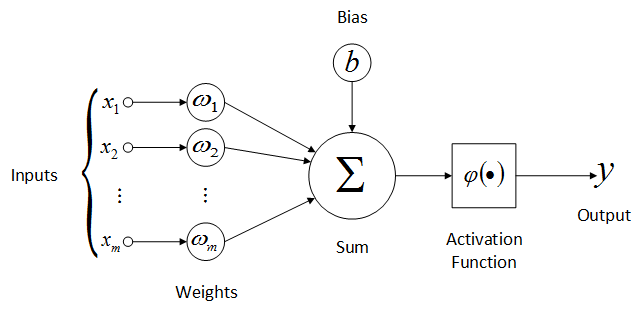
\includegraphics[width=0.8\textwidth]{images/neuron.png}
	\caption{Visualisierung eines künstlichen Neurons definiert nach der Gleichung \ref{eq:neuron}. Dieser Neuron summiert das Produkt des Inputvektors $x$  mit den jeweiligen Gewichten $w$ und addiert einen Bias $b$. Durch die Summe erzeugt die Aktivierungsfunktion $\phi$ das Output $y$ des Neurons. Entnommen aus \cite{deoliveiraSystemBasedArtificial2017}. }
	\label{fig:neuron}
\end{figure}

\subsubsection{Feedforward Neural Networks}
\label{sec:feedforwardNN}
Künstliche Neuronen können zu einer Schicht (\textit{layer}) zusammengeführt werden. Verbindungen solcher Schichten bilden einen neuronales Netzwerk.
Bei einem \textit{feedforward} (\textit{fully-connected}) Netzwerk übergibt jedes Neuron aus der Schicht $l$ seinen Output $y_{l}$ an jedes Neuron der Schicht $l+1$ weiter. Ebenso sind Neuronen aus der gleichen Schicht untereinander nicht verbunden \cite{Goodfellow-et-al-2016}.
Eine Schicht $l$ eines feedforward Netzwerkes operiert somit auf das Ouput $y_{l-1}$ und stellt die nicht-lineare Funktion $f_l :  \mathbb{R}^{M_{l-1}} \mapsto \mathbb{R}^{M_l}$ dar \cite{bauckhageInformedMachineLearning}:
\begin{equation}
\label{eq:layer}
y_l = f_l(y_{l-1}) = \phi(W^T_lx_{l-1}+b_{l})
\end{equation}


Die erste Schicht eines Netzwerk wird als Input-, die letzte Schicht als Ouput-Layer bezeichnet. Alle Schichten dazwischen sind Hidden-Layer \cite{Goodfellow-et-al-2016}. Der Ouput-Layer liefert zugleich auch das Ergebniss eines Netzwerks, daher haben die Neuronen des Ouput-Layers meist keine Aktivierungsfunktion \cite{CS231nConvolutionalNeural}.

Die Tiefe (\textit{depth}) eines Netzwerks ist gegeben durch die Anzahl der Layers \footnote{der Input-Layer ist ausgeschloßen} und die Breite (\textit{width}) eines Layers wird durch die Anzahl der Neuronen bestimmt \cite{Goodfellow-et-al-2016}. 
Abilldung \ref{fig:neural_net} illustriert ein feedforward neuronales Netz als ein azyklischer Graph.

Ziel eines KNNs ist es eine Funktion $f^*$ zu approximieren, dass einen Input $x$ auf einen Output $y$ abbildet. Durch das Output $y$ kann das Input $x$ klassifiziert oder ein Wert regressiert werden. Sei $y = f(x; \theta)$  solch eine Funktion, dann besetzt ein KNN die Werte des $\theta$ Parameters mit eines der besten Approximierung. Der Parameter $\theta$ stellt hierbei die Gewichte dar, welche erlernt werden sollen \cite{Goodfellow-et-al-2016}. 
Das Lernen ist die strategische Anpassung der Gewichte über Input-Output Paare (\textit{Trainingsdaten}) und findet i.d.R. durch ein \textit{Backpropagation}-Verfahren statt \cite{Goodfellow-et-al-2016}. 

Die Funktion $y = f(x; \theta)$ bildet sich aus den Funktionen der Schichten (Gleichung \ref{eq:layer}) im Netzwerk und kann bei einer Tiefe $L$ repräsentiert werden als die folgende Funktion $f :  \mathbb{R}^{M_0} \mapsto \mathbb{R}^{M_L}$ \cite{Goodfellow-et-al-2016, bauckhageInformedMachineLearning}:
 
\begin{equation}
\label{eq:network}
y = f(x; \theta)=  f_L(...f_2(f_1(x))) = (f_L \circ ... \circ f_2 \circ f_1)(x)
\end{equation}

\begin{figure}[H]
	\centering
	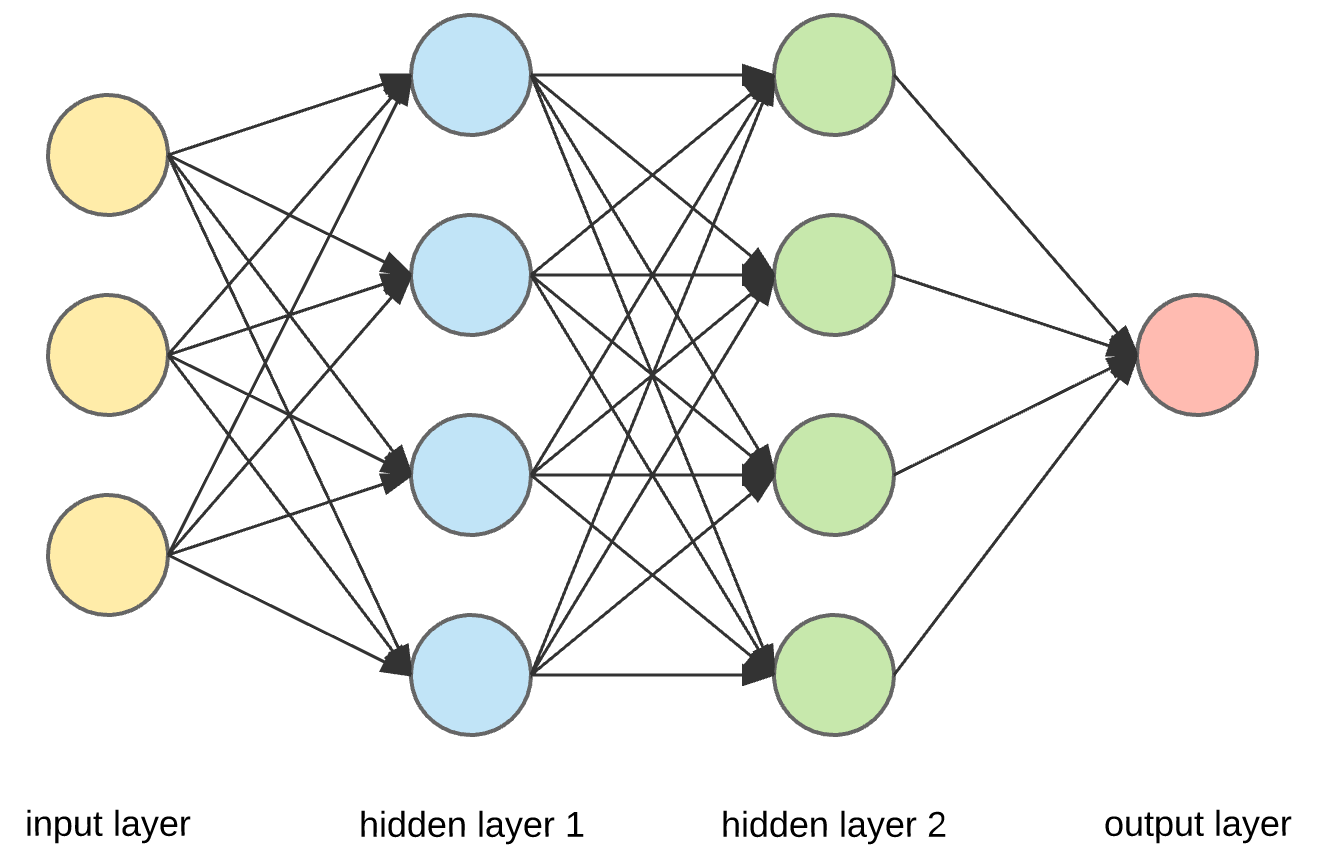
\includegraphics[width=0.6\textwidth]{images/neural_net.png}
	\caption{Ein feedforward neuronales Netz mit der Tiefe 3 bestehend aus einem Input-Layer der Breite 3, aus zwei Hidden-Layer der Breite 4 und einem Output-Layer der Breite 1. Mit der Gleichung \ref{eq:network}  lässt sich dieses Netzwerk als die Funktion $f :  \mathbb{R}^{3} \mapsto \mathbb{R}^{1}$ mit $f(x)=f_3(f_2(f_1(x)))$ darstellen. }
	\label{fig:neural_net}
\end{figure}

\subsection{Convolutional Neural Networks}

Einfache neuronale Netze, wie sie in Abschnitt \ref{sec:KNN} beschrieben wurden, arbeitet auf einem Inputsvektor $x \in \mathbb{R}^{M}$. Hingegen arbeiten CNNs auf einem drei-dimensionalen Inputsvolumen $x \in \mathbb{R}^{width} \times \mathbb{R}^{heigth} \times \mathbb{R}^{depth}$. CNNs werden hauptsächlich im Kontext von Bildern eingesetzt, dabei stellt z.B. ein 32 $\times$ 32 RGB-Bild ein Volumen von 32 $\times$ 32 $\times$ 3 dar \cite{CS231nConvolutionalNeurala}.

Eine Convolutional Neural Network Architektur setzt sich aus einer Sequenz von unterschiedlichen Schichtarten zusammen \cite{CS231nConvolutionalNeurala}. Im weiteren Verlauf dieses Kapitels werden die Arten der Schichten beschrieben. Tabelle \ref{tab:layer_param} gibt eine Übersicht der Schichten und Ihrer Parameter an.

\begin{table}
	\centering
	\caption{Übersicht der Paramter und Hyperparamter der Schichten eines Convolutional Neural Networks. Parameter werden während der Trainingsphase optimiert und Hyperparameter werden vorab fest definiert \cite{yamashitaConvolutionalNeuralNetworks2018}. }
	\begin{tabularx}{0.9\textwidth}{X X X}
		\textbf{Art des Schichtes} & \textbf{Parameter} & \textbf{Hyperparameter}\\
		\hline
		Convolutional Layer & Filter & \makecell[tl]{
			Anzahl der Filter\\
			Filtergröße\\
			Stride\\
			Padding\\
			Aktivierungsfunktion
		}\\
		\hline
		Pooling Layer &  \textit{keine}  & \makecell[tl]{
			Pooling Methode\\
			Filtergröße\\
			Stride\\
			Padding
		}\\
		\hline
		Fully-Connected Layer & Gewichte & \makecell[tl]{
			Anzahl der Gewichte\\
			Aktivierungsfunktion
		}\\
		\hline
	\end{tabularx}
	\label{tab:layer_param}
\end{table}


\begin{figure}[h]
	\centering
	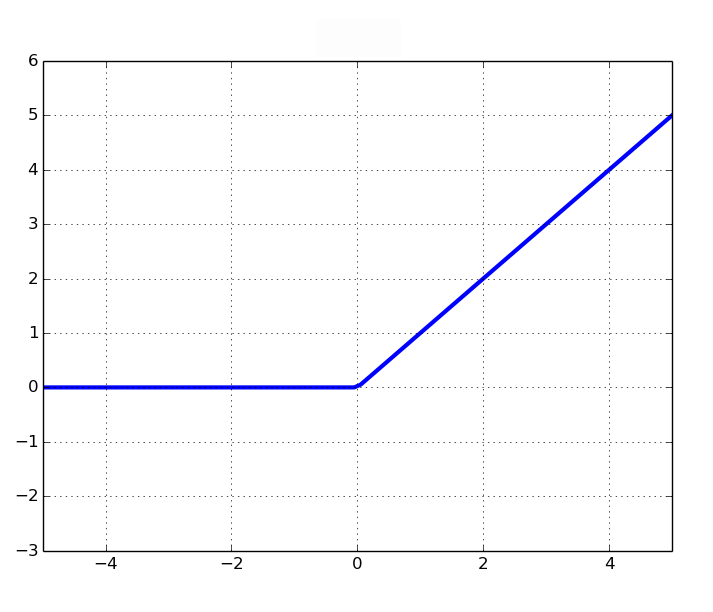
\includegraphics[width=0.4\textwidth]{images/ReLU.png}
	\caption{Ein Beispiel für eine Aktivierungsfunktion. Die ReLU (\textit{rectified liniear unit}) Aktivierungsfunktion wird typischerweise in CNNs eingesetzt und ist mathematisch definiert als: $f(x) = max(0,x)$ \cite{Goodfellow-et-al-2016} }
	\label{fig:relu}
\end{figure}

\subsubsection{Convolution Layer}
Der Convolutional Layer ist der Hauptbestandteil eines CNNs, welches die Kombination eines Convolution Operationen und einer Aktivierungsfunktion ist \cite{yamashitaConvolutionalNeuralNetworks2018}.
\begin{figure}[H]
	\centering
	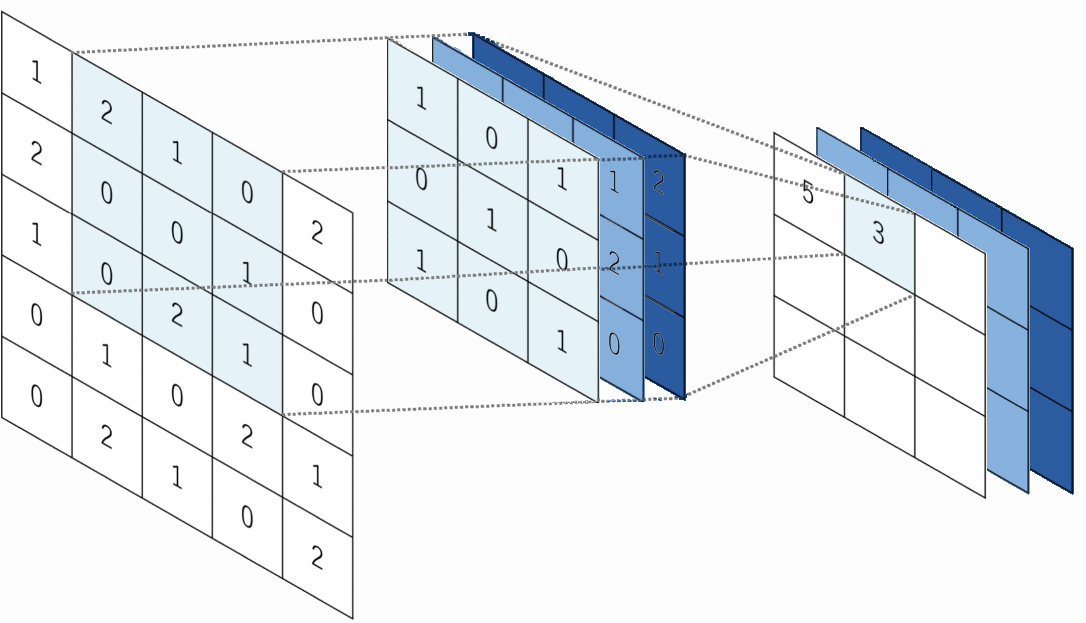
\includegraphics[width=0.7\textwidth]{images/convolution_layer.png}
	\caption{Ein Beispiel für die  Convolution Operation mit 3 Filtern der Größe 3 $\times$ 3, einem Stride von 1 und keinem Padding. Ein Filter bewegt sich entlang des gesamten Inputs mit der Schrittweite \textit{Stride} und bildet die Summe der elementweise multiplizierten Werte. Die Summe wird dann im Output an die korrespondierende Position geschrieben. Dieser Vorgang wiederholt sich für jedes Filter. \cite{yamashitaConvolutionalNeuralNetworks2018}. }
	\label{fig:convolution_layer}
\end{figure}
\newpage
\subsubsection{Pooling Layer}
Auf einen Convolutional Layer folgt i.d.R. ein Pooling Layer. Pooling Layer reduzieren die Größe eines Inputsvolumen und verringert somit die Anzahl der erlernbaren Parameter. Die Pooling Operation wird auf jeder Schicht der Eingabe ausgeführt \cite{CS231nConvolutionalNeurala}. Die meist verbreitete Pooling Operation ist die Max-Pooling. Beim Max-Pooling wird der Input in Bereiche einer bestimmten Filtergröße eingeteilt und nur der Maximum der Bereiche für die weitere Berechnung beibehalten und die restlichen Werte verworfen
 \cite{CS231nConvolutionalNeurala}. In dieser Arbeit wird neben der Max-Pooling Operation auch die Average-Pooling Operation eingesetzt. Das Average-Pooling behält je Bereich den Durchschnittswert, statt den Maximum \cite{CS231nConvolutionalNeurala}.
 
 Im Vergleich zu einem Convolutional Layers wird ein Pooling Layer nur aus Hyperparametern definiert und bleibt daher statisch \cite{yamashitaConvolutionalNeuralNetworks2018}. Abbildung \ref{fig:pooling_layer} zeigt eine beispielhafte Ausführung einer Max-Pooling Operation. Tabelle \ref{tab:layer_param} listet die Hyperparameter eines Pooling Layers auf.
 \begin{figure}[H]
	\centering
	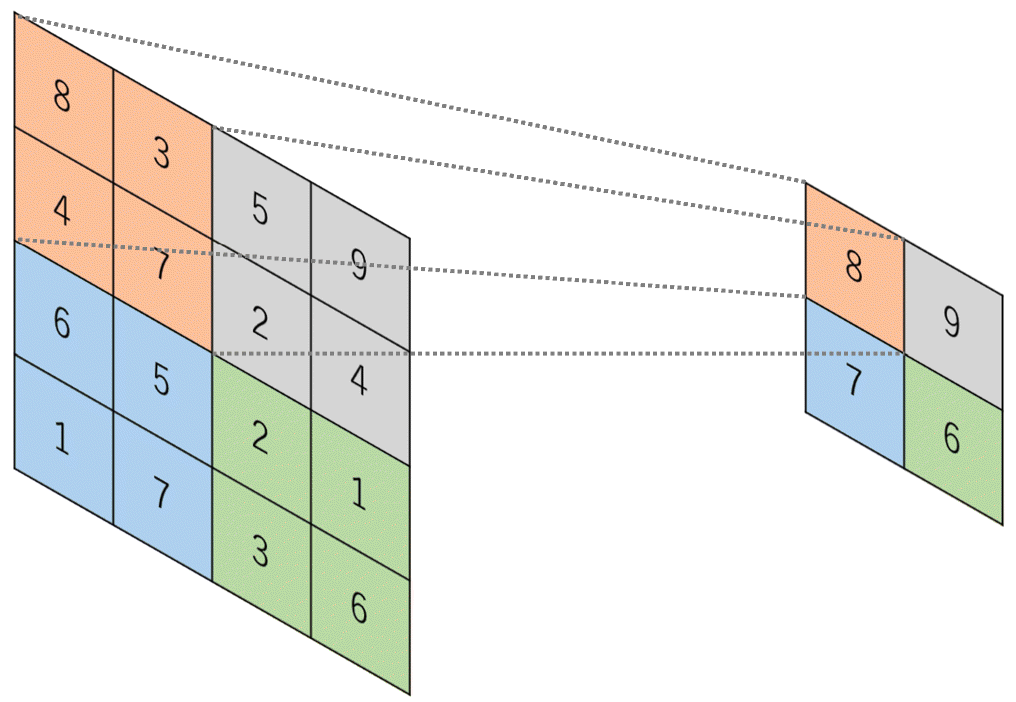
\includegraphics[width=0.6\textwidth]{images/max_pool.png}
	\caption{Ein Beispiel für eine Max-Pooling Operation mit einer Filtergröße von 2 $\times$ 2, einem Stride von 2 mit keinem Padding. In diesem Beispiel wird der Input in 2 $\times$ 2 Bereiche unterteilt und der Maximum jedes Bereiches als Output berechnet. Es werden die markantesten Werte einer Nachbarschaft behalten und der Rest verworfen. Diese Operation führt zu einer Reduzierung der Inputgröße um den Faktor 2. Entnommen aus \cite{yamashitaConvolutionalNeuralNetworks2018}.}
	\label{fig:pooling_layer}
\end{figure}



\subsubsection{Fully-Connected Layer}
Nach einer Periode von Convolution und Pooling Layers folgt meist eine fully-connected Layer, auch bekannt als \textit{Dense Layer}. Dieser Layer folgt den gleichen Konzept, wie in Abschnitt \ref{sec:feedforwardNN} beschrieben. Der Output dieses Layers wird meist einer weiteren Aktivierungsfunktion übergeben \cite{yamashitaConvolutionalNeuralNetworks2018} und i.d.R. wird durch die Aktivierungsfunktion der Output des CNNs bestimmt.

\subsection{Bekannte CNN Modelle}
\subsubsection{GoogLeNet}
\subsubsection{PoseNet}

\pagebreak